
\section{Raspberry Pi - Google Assistant}

Głównym elementem naszego projektu jest mikrokomputer Raspberry Pi 3 w wersji B. Zostanie na nim zainstalowany serwer aplikacji webowej (omówiony w rozdziale <tu wstaw rozdział> i Google Assistant. W niniejszej części dokumentu zostanie omówiony projekt bezpośredniego połączenia Raspberry Pi z urządzeniami zewnętrznymi (takimi jak głośnik, mikrofon) stanowiącymi razem pewną integralną całość, w założeniu mającą znaleźć się w jednej obudowie. Zdalny moduł wykorzystujący ESP8266 zostanie omówiony w innej części tego dokumentu.

\subsection{Spis urządzeń}

\begin{enumerate}
\item Raspberry Pi 3 w wersji B \\
	\begin{center}
	\adjustbox{valign=t}{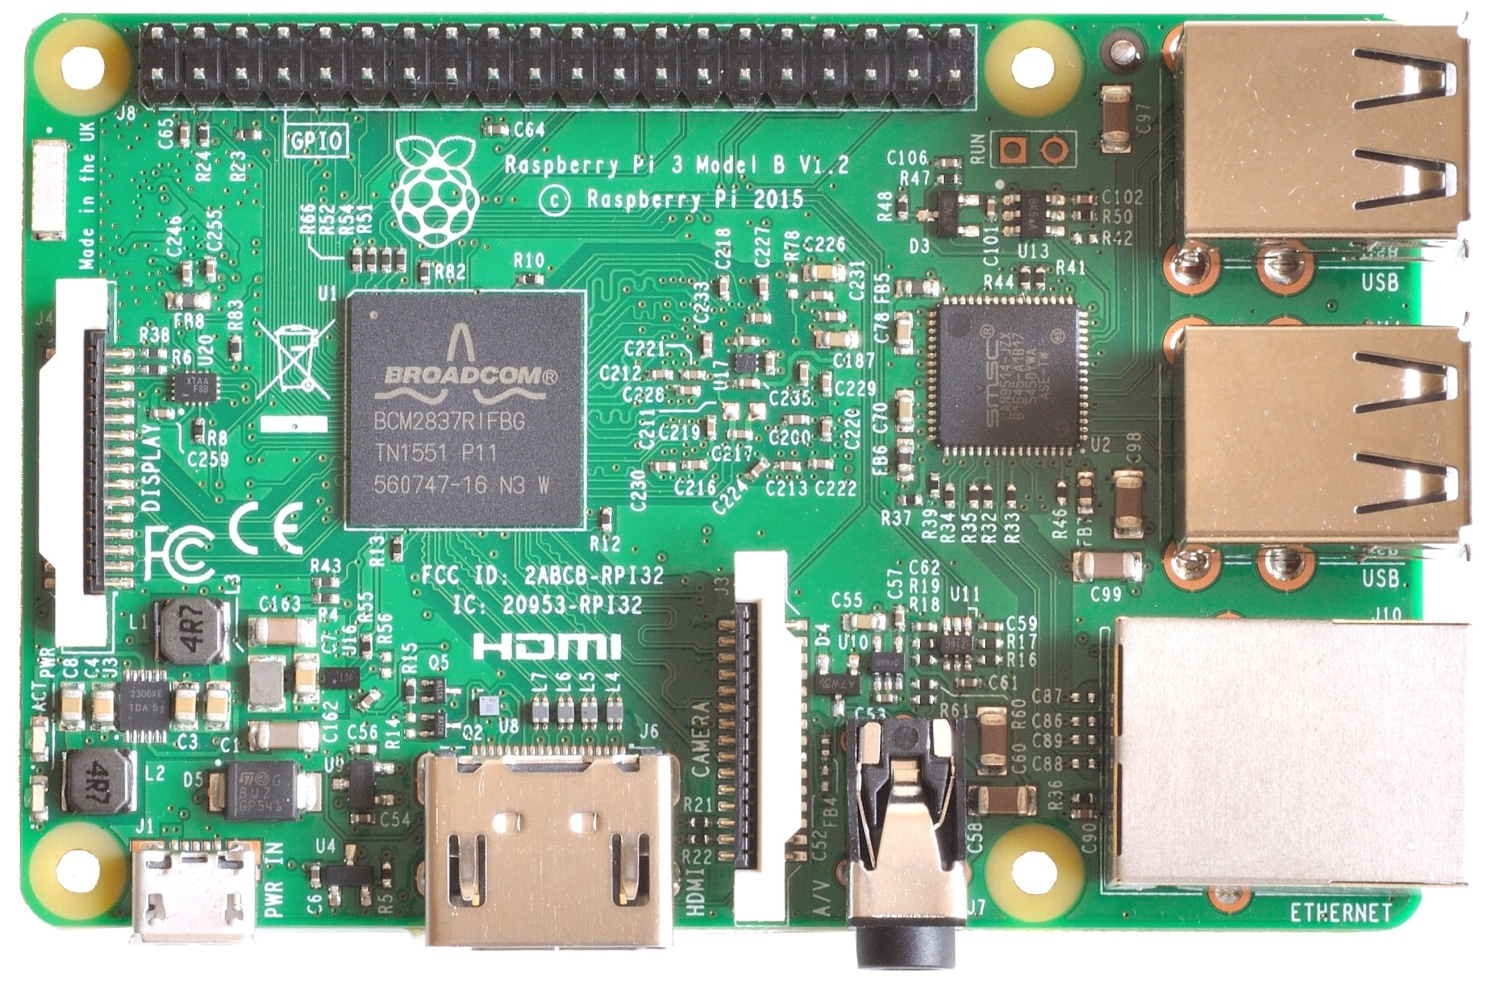
\includegraphics[width=10cm]{rpi.jpg}}
	\end{center}
\item Zewnętrzna karta dżwiękowa Virtual 7.1 Channel USB \\
	\begin{center}
	\adjustbox{valign=t}{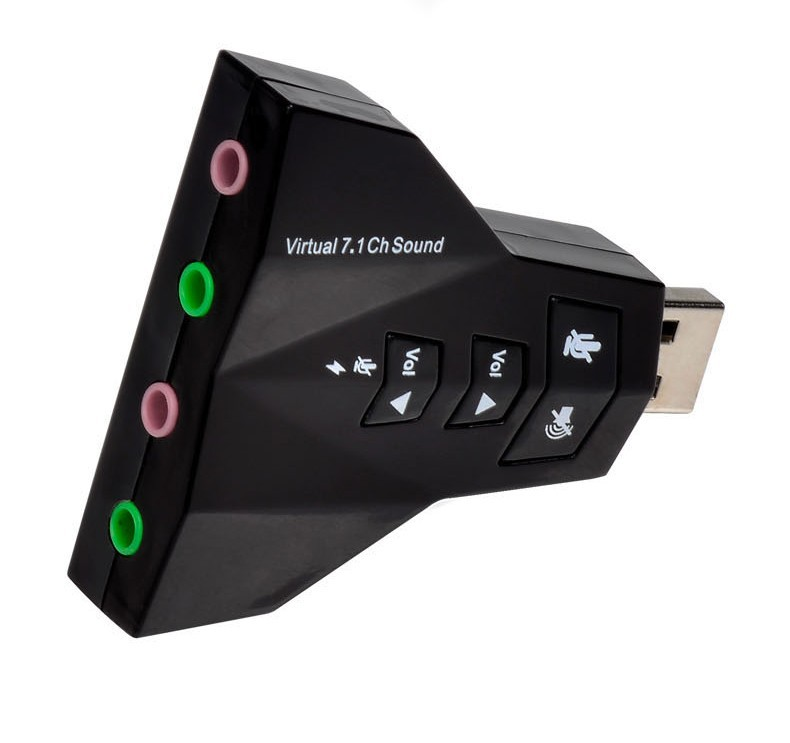
\includegraphics[width=10cm]{karta_muzyczna.jpg}}
	\end{center}
\item Głośnik 3W 8Ohm 40x88mm \\
	\begin{center}
	\adjustbox{valign=t}{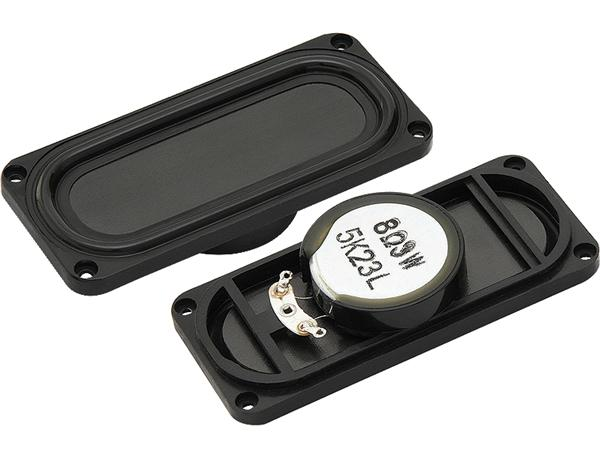
\includegraphics[width=10cm]{glosnik.jpg}}
	\end{center}
\item Wzmacniacz audio stereo PAM8403 5V 3W - dwukanałowy \\
	\begin{center}
	\adjustbox{valign=t}{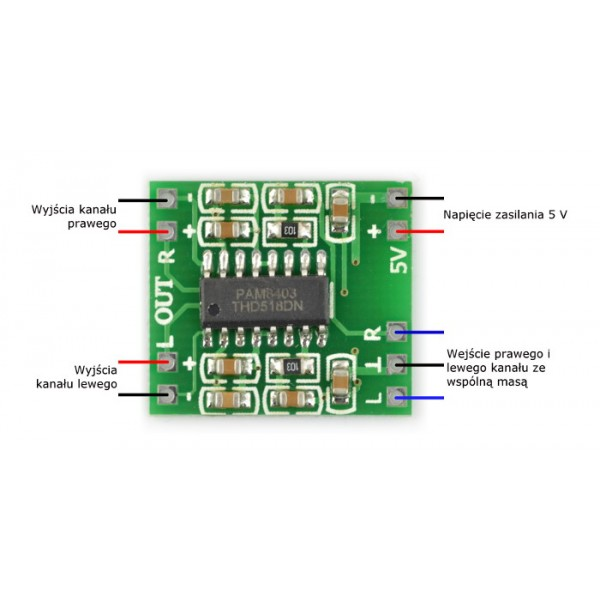
\includegraphics[width=10cm]{wzmacniacz.jpg}}
	\end{center}
\item Przycisk Arcade Push Button niebieski z podświetleniem \\
	\begin{center}
	\adjustbox{valign=t}{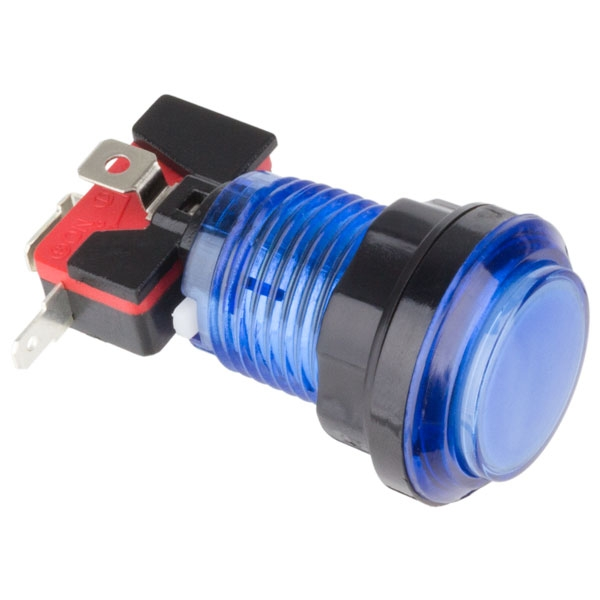
\includegraphics[width=10cm]{button.jpg}}
	\end{center}
\item mikrofon
\end{enumerate}

\subsection{Schemat połączeń}

Na poniższym schemacie zaprezentowano układ połączeń wyżej wymienionych elementów. Rezystancje oporników mogą się różnić ze względu na wykorzystany tranzystor i rodzaj diody świecącej. W większości przypadków układ typu "klucz npn" nie będzie potrzebny, gdyż napięcie przewodzenia diody może okazać na tyle niskie, że będzie możliwe zasilenie jej z portu GPIO (niestety nie było tak w naszym przypadku).

\begin{center}
\adjustbox{valign=t}{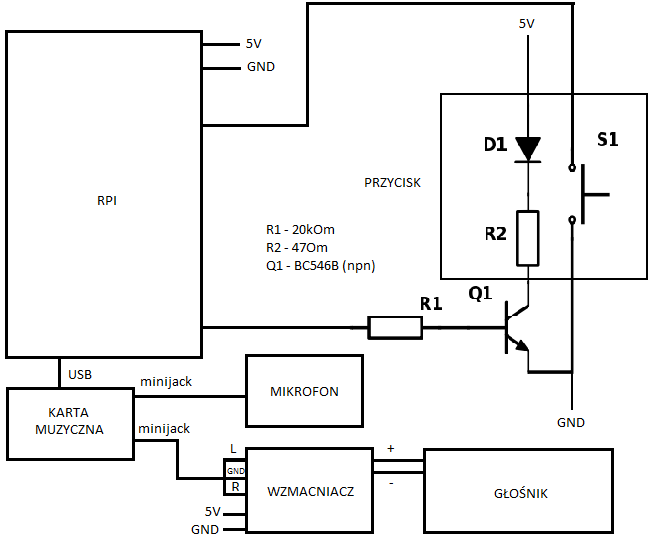
\includegraphics[width=10cm]{schematRPI.png}}
\end{center}


\section{ESP8266}

Drugim kluczowym elementem naszego projektu jest układ wykorzystujący moduł \emph{ESP8266}. Zostanie do niego podłączony nadajnik IR, odbiornik IR i bateria. Gdy odczyt sygnału, nadawanego przez pierwsze z urządzeń, nie będzie możliwy, znaczy to, że na drodze wiązki znajduje się jakaś przeszkoda - w założeniach ma to być list. Moduł zostanie oprogramowany tak aby, co jakiś ustalony czas, wysyłać do serwera informacje o odczycie. W finalnej wersji układ ma zostać zamontowany w skrzynce.
\subsection{Spis urządzeń}

\begin{enumerate}
	\item ESP8266 z ModeMCU v3 \\
	\begin{center}
		\adjustbox{valign=t}{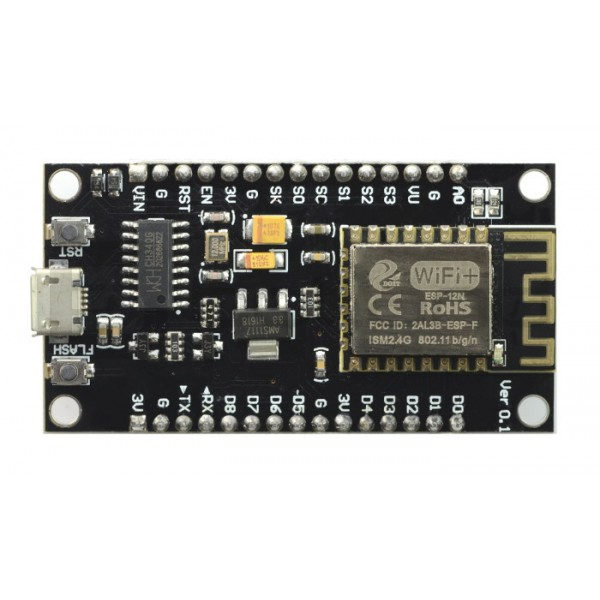
\includegraphics[width=10cm]{esp8266-nodemcu-v3.jpg}}
	\end{center}
	\item Odbiornik TSOP4836 \\
	\begin{center}
		\adjustbox{valign=t}{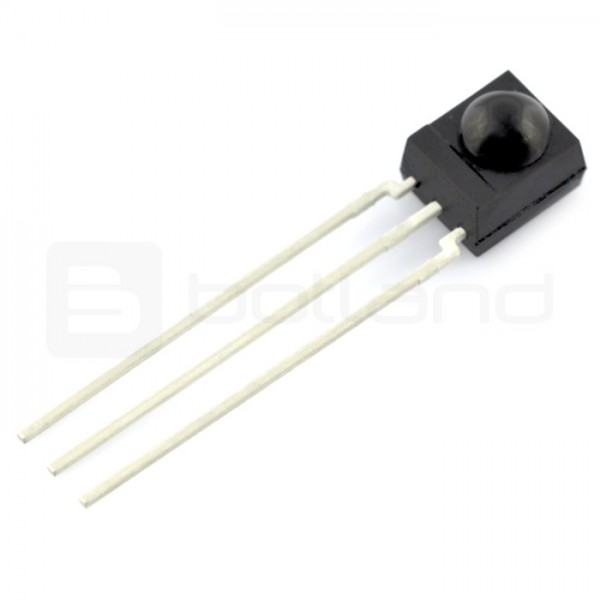
\includegraphics[width=10cm]{tsop4836.jpg}}
	\end{center}
	\item Nadajnik IR LIRED5C \\
	\begin{center}
		\adjustbox{valign=t}{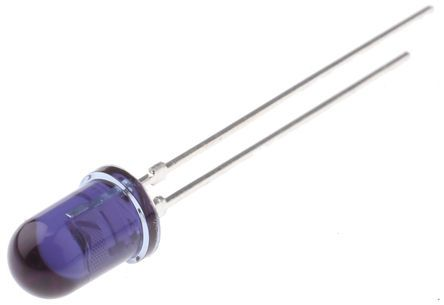
\includegraphics[width=10cm]{LIRED5C.jpg}}
	\end{center}
\end{enumerate}

\subsection{Schemat połączeń}

Poniższy schemat przedstawia układ połączeń wyżej wymienionych elementów. Warto zwrócić uwagę na połączenie pinu GPIO\_16 z pinem REST. Pozwoli to przełączać moduł ESP w tryb głębokiego snu - pozwoli to na oszczędzanie baterii.

\begin{center}
	\adjustbox{valign=t}{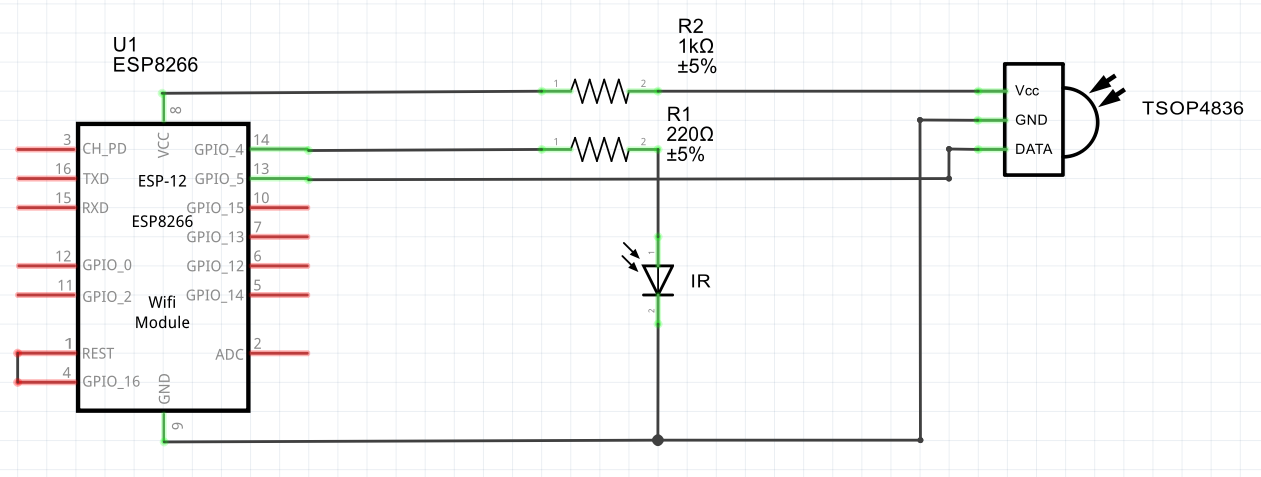
\includegraphics[width=10cm]{schematWiFI_IR.png}}
\end{center}

\section{Serwer}

Następną częścią projektu jest serwer oparty o technologię \textit{Flask}. Pozwala on na komunikację pomiędzy \textit{ESP8266}, \textit{Google Assistantem} oraz aplikacją webową.\\

Serwer jest uruchamiany na \textit{Raspberry PI}, na porcie 5000 i udostępnia klientom dwa \textit{endpointy}. Jeden z nich pozwala na pobranie aktualnego stanu skrzynki pocztowej, drugi - na jego zmianę. \\

Stan skrzynki jest zapisywany w pliku, w postaci:
\begin{itemize}
\item 0 - gdy skrzynka jest pusta
\item 1 - gdy w skrzynce mamy jakieś wiadomości
\end{itemize}

W przypadku, jeśli na \textit{Raspberry PI} nie ma wymaganych przez serwer zależności (Flask w wersji 0.10.1) należy wywołać:
\begin{lstlisting}
pip install -r requirements.txt
\end{lstlisting}

Uruchamianie serwera następuje przez wywołanie:
\begin{lstlisting}
python run.py
\end{lstlisting}


\section{Aplikacja webowa}

\begin{center}
	\label{img:skrzynka}
	\adjustbox{valign=t}{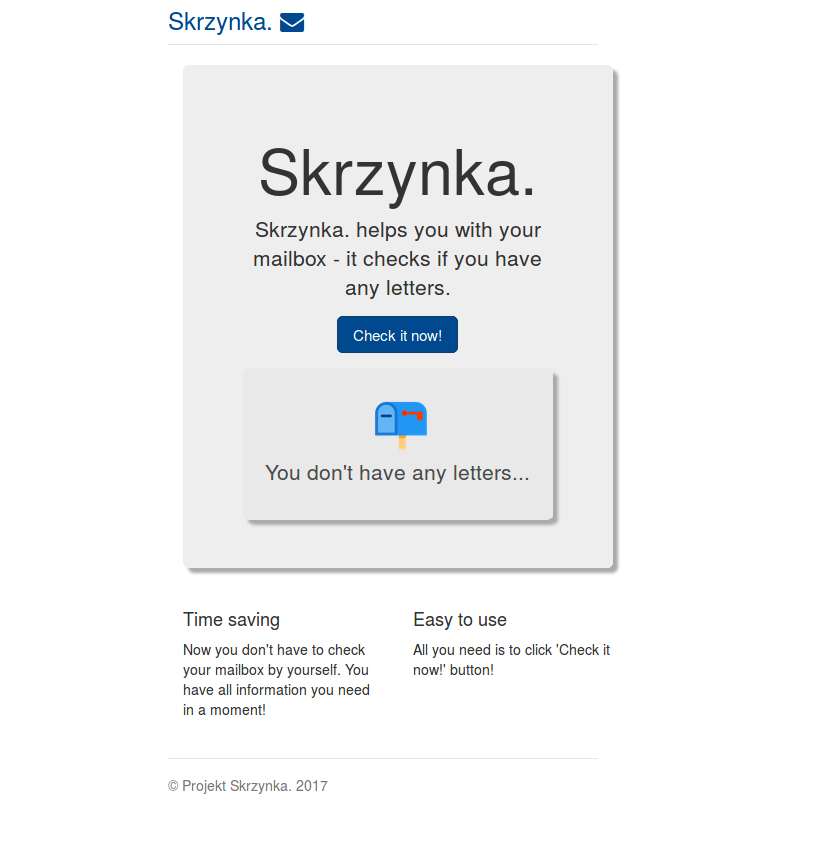
\includegraphics[width=10cm]{skrzynka.png}}
\end{center}

Aplikacja webowa pozwala na sprawdzenie aktualnego stanu skrzynki pocztowej. Jest widoczna na rysunkach \ref{img:skrzynka} i \ref{img:skrzynka2}.
Logika aplikacji została stworzona w języku \textit{Java Script} wraz z \textit{AngularJS}, natomiast widok to \textit{HTML5} wraz z arkuszami stylów (\textit{CSS}).\\

Składa się z trzech głównych części:
\begin{itemize}
\item widoku - który określa elementy, jakie są obecne na stronie
\item kontrolera - który odpowiada za logikę w aplikacji (wykorzystuje serwis do wysyłania zapytań do serwera)
\item serwisu - który wysyła zapytanie \textbf{GET /state} na adres serwera
\end{itemize}

Na stronie dostępny jest przycisk \textbf{Check it now!} (ang. \textit{Wypróbuj już teraz!}), który wywołuje metodę kontrolera odpowiedzialną za wykonanie zapytania do serwera przez serwis.

Uruchomienie serwera \textit{node.js} z parametrem wskazującym na ścieżkę do pliku \textbf{server.js}:
\begin{lstlisting}
node server.js
\end{lstlisting}

W przypadku, jeśli na \textit{Raspberry PI} nie ma wymaganych przez aplikację zależności należy wywołać:
\begin{lstlisting}
bower install
npm install connect
npm install serve-static
\end{lstlisting}
i później uruchomić serwer \textit{node.js}.

\begin{center}
	\label{img:skrzynka2}
	\adjustbox{valign=t}{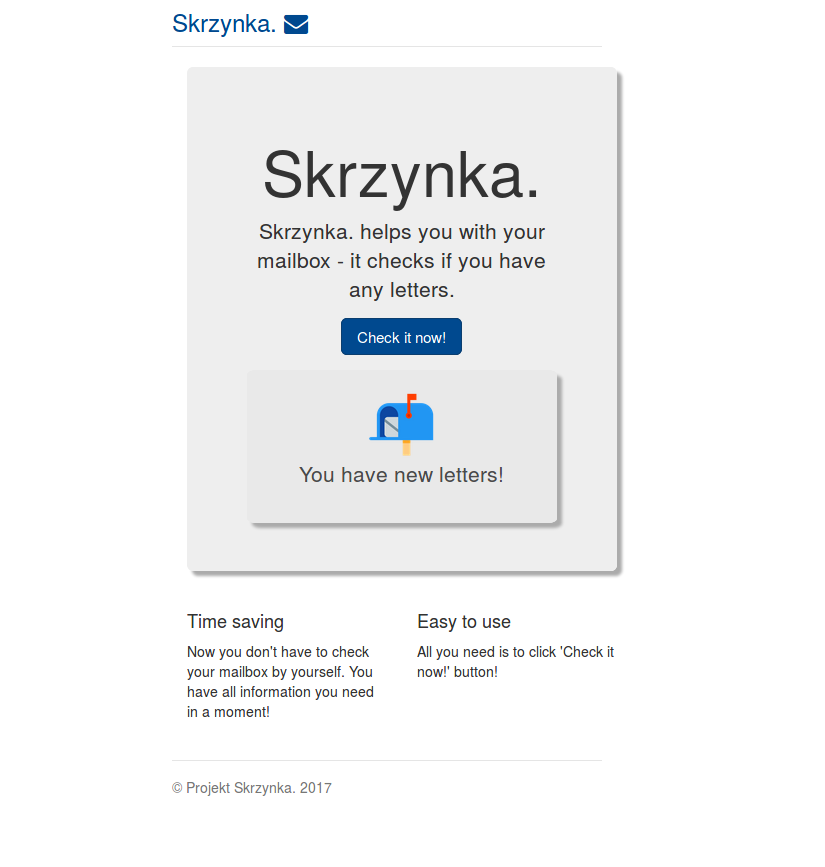
\includegraphics[width=10cm]{skrzynka2.png}}
\end{center}

